\documentclass{standalone}
\usepackage{tikz}
\usepackage{ctex,siunitx,bm}
\setCJKmainfont{Noto Serif CJK SC}
\usepackage{tkz-euclide,ninecolors}
\usepackage{amsmath}
\usetikzlibrary{patterns, calc}
\usetikzlibrary {decorations.pathmorphing, decorations.pathreplacing, decorations.shapes,}
\begin{document}
\small
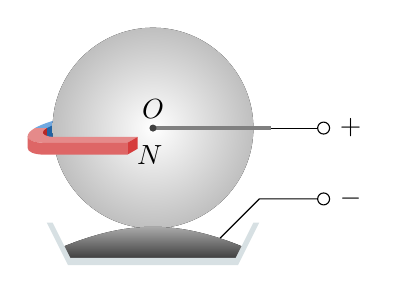
\begin{tikzpicture}[>=latex,scale=1.5]
  \fill[azure7](-0.900,0.000)..controls(-0.835,0.038)and(-0.670,0.075)..(-0.570,0.075)--(-0.483,0.125)..controls(-0.633,0.125)and(-0.892,0.062)..(-1.000,0.000)--cycle;
  \fill[azure4](-0.900, 0.000)..controls(-0.835, 0.038)and(-0.670, 0.075)..(-0.570, 0.075)--(-0.570,-0.025)..controls(-0.670,-0.025)and(-0.835,-0.062)..(-0.900,-0.100)--cycle;
  \fill[outer color=lightgray,inner color=white](0,0)circle(0.85);
  \fill[red4](-0.900, 0.000)rectangle(-0.95,-0.1);
  \fill[red7](-1.000, 0.000)..controls(-1.042,-0.024)and(-1.061,-0.048)..(-1.061,-0.069)..controls(-1.061,-0.101)and(-1.009,-0.125)..(-0.917,-0.125)--(-0.217,-0.125)--(-0.130,-0.075)--(-0.830,-0.075)..controls(-0.868,-0.075)and(-0.896,-0.070)..(-0.914,-0.061)..controls(-0.942,-0.047)and(-0.940,-0.023)..(-0.900, 0.000)--cycle;
  \fill[red6](-1.061,-0.169)..controls(-1.061,-0.201)and(-1.009,-0.225)..(-0.917,-0.225)--(-0.217,-0.225)--(-0.217,-0.125)--(-0.917,-0.125)..controls(-1.009,-0.125)and(-1.061,-0.101)..(-1.061,-0.069)--cycle;
  \fill[red5](-0.130,-0.075)--(-0.130,-0.175)--(-0.217,-0.225)node[text=black,right]{$N$}--(-0.217,-0.125)--cycle;
  \fill[gray](0,-0.02)rectangle(1,0.02);
  \fill[darkgray](0,0)circle(0.03)node[above,text=black]{$O$};
  \draw[-o](1,0)--(1.5,0)node[right]{$+$};
  \draw[-o](0.5,-1.0)--(0.9,-0.6)--(1.5,-0.6)node[right]{$-$};
  \fill[top color=lightgray,bottom color=darkgray](-0.7,-1.1)--(-0.75,-1.0)to[bend left=22](0.75,-1.0)--(0.7,-1.1);
  \fill[cyan!20!gray!30](-0.7,-1.1)--(-0.85,-0.8)--++(-0.05,0)--++(0.18,-0.36)--++(1.44,0)--++(0.18,0.36)--++(-0.05,0)--(0.7,-1.1);
\end{tikzpicture}
\end{document}